\documentclass{article}
\usepackage[utf8]{inputenc}
\usepackage{hyperref}
\title{keccak preimage}
\usepackage{graphicx}
\usepackage{tikz}
\usepackage{tikz,graphicx}
\usepackage[absolute,overlay]{textpos} 
\usetikzlibrary{decorations.pathmorphing,matrix,decorations.pathreplacing,arrows,decorations.markings}
\usetikzlibrary{fit,calc,shapes,arrows,positioning,shadings,backgrounds,patterns,tikzmark,matrix,spy}
\usetikzlibrary{decorations.markings}

\usepackage[T1]{fontenc}
\begin{document}

\maketitle

\section{Introduction}

The observations based on the following paper : \textbf{Linear Structures: Applications to Cryptanalysis of Round-Reduced Keccak}.

\subsection{2R Keccak-512}

See Fig. 8, for each guess :
we set 
\[
    A[0, 1] = A[0, 0] \oplus \alpha_{0}
\]
\[
    A[2, 1] = A[2, 0] \oplus \alpha_{2}
\]
with $\alpha_0$ and $\alpha_2$ as random constants

Since $A[0,0]$ and $A[2,0]$ have 128 bits. So we have a complexity gain over bruteforce of $2^{128}$. Hence the time complexity $= 2^{512 - 128} = 2^{384}$.

Input degree of freedom : 
\begin{enumerate}
    \item 64 bits from $A[0, 0]$ , 64 bits from $A[2,0]$.
    \item (320 -1) bits from white lanes
    \item 128 bits from $\alpha_0, \alpha_2$
\end{enumerate}

This sums upto 575 bits larger than required 512 bits.

\subsection{2R Keccak-384}

\begin{enumerate}
    \item Attack similar to Keccak-512
    \item Can obtain a linear structure of 256 bits variables from 
    \[
        (A[0, 0], A[0, 1], A[2, 0], A[2, 1])
    \]
    
    \item with : $A[0, 2] = A[0, 0] \oplus A[0, 1] \oplus \alpha_0$
    \item and $A[2, 2] = A[2, 0] \oplus A[2, 1] \oplus \alpha_2$
    \item Hence a linear system of 256-bit equations
    \item Msg satisfying padding rule, need a solution with the last bit of A[2,2] being 1
    \item Time Complexity of Attack $ = 2^{384 - 256 + 1} = 2^{129}$
\end{enumerate}

\textbf{Note :} In the following document WM refers to Willi Meier

\section{Suggestion by WM}

\subsection{Mail : 5 Feb}

Mail contents are : 
\begin{quote}
    I mainly refer to : https://eprint.iacr.org/2016/878
    
    We try to loosen restrictions imposed by linear structures to increase freedom degrees.
    
    An example is 2-round Keccak-384. I refer to Fig. 9. In addition to the colored 6 lanes that are variable, we also keep lanes 3,0 and 3,1 variable, still so that sum of columns is kept constant. Then $\chi$ produces one quadratic lane. We substitute quadratic monomials by 64 linear variables.
    
    We can invert the first row of image (green), and we require that the map to the 6-th green lane is linear (i.e. quadratic part happens to vanish). The probability for this event is about $.75^{64} = 2^{27}$

    Then we have $ 4*64 + 64 + 64 = 384$ variables and the same number of conditions. Solving this linear system has about 1 solution, that we may check by substituting it into 2-round Keccak. Genuine number of freedom degrees is 320, and artficial ones 384. It is likely to find a correct solution in $2^{64} * 2^{27}= 2^{91}$ trials. This case was found in discussion with Meicheng Liu and Jian Guo.
    I believe that something similar (or better) will work for 2-round Keccak-512. In addition to substitution of a quadratic lane by linear variables, we know that variables in same column are linearly related. This means that in quadratic lanes after $\chi$, some linear factors  are essentially "the same".

    The probability of a1*a2 =a1*a3 is 0.75 for any values a1, a2, a3. We substitute monomials of the form a1*a2  and a1*a3 by the same linear variable to get more linear equations that will hold true with reasonable probability. We introduce artificial linear variables economically, so that we don't have more linear variables (genuine and artificial ones) than equations.Details need to be checked.
    
    Wonder whether this could also help, e.g., in 3-round Keccak-256 in \url{https://tosc.iacr.org/index.php/ToSC/article/view/802}.
    
    An issue is how far these observations extend to improve 3 round preimages of Keccak-384 and Keccak-512, as described in Sect. 6.3.
    
    As complexities of known preimages of 4-round Keccak-512 are still close to $2^{512}$, there is some slight hope that we might reach 4 rounds for this case.
    
    Do you have any comments on this?
    \end{quote}
    
    \begin{enumerate}
        \item Here in addition to Keccak-384 setting for 2 Round attack.
        \item In Fig. 9 we keep lanes (3, 0) and (3, 1) also as variables
        \item $A[3, 1] = A[3, 0] \oplus \alpha_3$ (so that sum of columns remains constant)
        \item Linear structure of 320-bit :
        \item $( A[0, 0], A[0, 1], A[2, 0], A[2, 1], A[3, 0] )$
        \item A quadratic term is introduced after 1st $\chi$ by product of $(2, 0), (3, 1)$ as both are variables.
        \item For this we substitute quadratic monomials by 64 linear variables.
        \item Now next problem was for last round : $(\chi o \iota)^{-1}$
        \item For the green lane of second row, this happens to be linear with probability $= 0.75$
        \item For 64 slices, this $= 0.75^{64}$, which adds $2^{27}$ trials
        \item Complexity comes out to be $ = 2^{64} * 2^{27} = 2^{91}$ trials.
        \item \textbf{ Comments : }
        \begin{enumerate}
            \item Any issue of Linear independent variable for solution of equations?
            \item Otherwise the analysis is fine here.
        \end{enumerate}
    \end{enumerate}
    \subsection{Suggestion for Keccak-384, 2R}
\begin{enumerate}
    \item \textbf{Note :} After verification this comes out to be incorrect
    \item Same as the setting introduced by WM for 2R Keccak-384 where we keep (3,0) and (3,1) also as variables
    \item Here we introduced a new variable for each quadratic term
    \item The suggestion here is for reducing the trials due to the last round linear $\chi$ inversion.
    \item Instead of inverting $\chi$ for 6th green lane as suggested by WM we can do something like this :
    \item \label{ob2}\textbf{Observation :} When only one output bit is known after $\chi$ step, then the corresponding input bits have $2^4$ possibilities. A way to fix the first output bit to be the same as input bit and the second bit as $1$. It is shown in the Figure~\ref{chi_inv2}.
\begin{figure}[ht]
\begin{center}
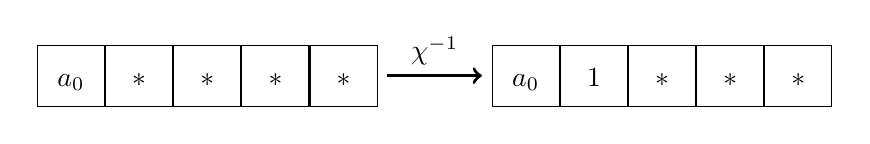
\begin{tikzpicture}[ampersand replacement=\&]
\matrix (m1) [matrix of nodes,
nodes={inner sep=5pt,text width=0.5cm,align=center,minimum height=.5cm, draw,text height=1em,text depth=.2em}
]{
	$a_0$ \& $*$ \& $*$ \& $*$ \& $*$\\
};

\matrix (m2) [right = 1.2cm of m1, matrix of nodes,
nodes={inner sep=5pt,text width=0.5cm,align=center,minimum height=.5cm, draw,text height=1em,text depth=.2em}
]{
	$a_0$ \& $1$ \& $*$ \& $*$ \& $*$\\
};
\draw[->, very thick] (m1)-- node[above, pos=0.5] {$\chi^{-1}$} (m2);
\end{tikzpicture}
\end{center}
\caption{Computation of $\chi^{-1}$\label{chi_inv2}}
\end{figure}
    \item Here in Fig. ~\ref{chi_inv2}, we fix the lane adjacent to 6th green lane as $1$ before $\chi$ operation. If this is assumed then the 6th lane is inverted as it is and seems like a constant.
    \item No. of variables : 5 lane variables + 1(substitute for quadratic terms) and 6 linear conditions. So we Linear structure : $(A[0,0], A[0,1], A[2, 0], A[2,1], A[3,0])$
    \item White lane (constants) : 5 lanes and $64*3$ bits from $\alpha_0, \alpha_2, \alpha_3$
    \item So the degree of freedom is much larger than required 384 bits.
    \item We just want a solution with last bit of $A[2,2]$ being 1.
    \item Time complexity = $2^{384 - (64*5) + 1} = 2^{65}$
    \item If this turns out to be correct then we have a much better attack than proposed by us in our indocrypt-2018 paper with complexity of $2^{88}$
    \item Please verify/correct this. If this is correct then something similar can also be applied to Keccak-512.
\end{enumerate}

\subsection{WM mail : 08/02/19}
For 2R Keccak-512 : 
\begin{enumerate}
    \item 1st row of hashes can be inverted
    \item For 2nd row, we know 3 consecutive outputs. So as in paper (Linear Structures: Applications to Cryptanalysis of Round-Reduced Keccak)
    \item Using table 4, we know that for 3 consecutive output bits in a row known we get 2 linear equations.
    \item For 64 lane size, we get $ 2*64 = 128 $ equations.
    \item For the Message : we keep columns 0, 1, 2 and 3 as variables
    \item \[ A[0, 1] = A[0, 0] \oplus \alpha_0 \]
        \[ A[1, 1] = A[1, 0] \oplus \alpha_1 \]
         \[ A[2, 1] = A[2, 0] \oplus \alpha_2 \]
         \[ A[3, 1] = A[3, 0] \oplus \alpha_3 \]
    \item This state produces quadratic variables after $\pi \circ \rho \circ \theta$.
    \item  This creates 3 quadratic lanes after $\chi$ of 1st round, caused by product of [0,0] with [1,1], and [1,0] with [2,1], and [2,0] with [3,1].
    \item Substitute each of the above quadratic variable by a new linear variable.
    \item So we need $3*64$ new linear variables
    \item Degree of freedom : 
    \begin{enumerate}
        \item Linear structure : $( A[0,0], A[1,0], A[2,0], A[3,0] )$ i.e. $4*64$ variables
        \item Artificial : $3*64$ linear variables
        \item Adds upto overall : $7*64$
    \end{enumerate}
    \item No. of linear conditions :
    \begin{enumerate}
        \item 5 from inversion of chi from the first row of hashes
        \item 2 from inversion of chi from 3 consecutive output bits of hash
        \item Hence, overall 7 equations
    \end{enumerate}
    \item We have 7 linear variables and 7 equations so we can expect to find a solution.
    \item But Actual degree of freedom : 4 i.e. $( A[0,0], A[1,0], A[2,0], A[3,0] )$ and 8 conditions on the final hash (8 lanes)
    \item So, no. of trials $= 2^{512 - 4*64} = 2^{64*4} = 2^{256}$
\end{enumerate}

\subsection{Suggestion for Keccak-384, 2R}
\begin{enumerate}
    \item Same as the setting introduced by WM for 2R Keccak-384 where we keep (4,0) and (4,1) also as variables
    \item Here we introduced two new variable for the quadratic terms.
    \item 2 quadratic lanes after $\chi$ of 1st round, caused by product of (4,0), (0,1) and (4,1), (0,2).
    \item The suggestion here is for reducing the trials due to the last round linear $\chi$ inversion.
    \item Instead of inverting $\chi$ for 6th green lane as suggested by WM we can do something like this :
    \item \label{ob2}\textbf{Observation :} When only one output bit is known after $\chi$ step, then the corresponding input bits have $2^4$ possibilities. A way to fix the first output bit to be the same as input bit and the second bit as $1$. It is shown in the Figure~\ref{chi_inv2}.
\begin{figure}[ht]
\begin{center}
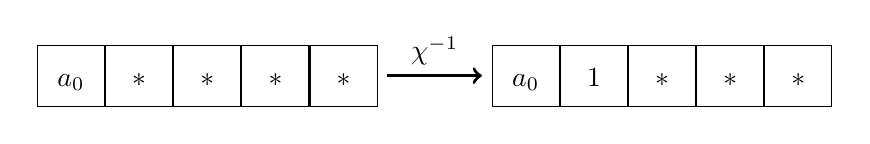
\begin{tikzpicture}[ampersand replacement=\&]
\matrix (m1) [matrix of nodes,
nodes={inner sep=5pt,text width=0.5cm,align=center,minimum height=.5cm, draw,text height=1em,text depth=.2em}
]{
	$a_0$ \& $*$ \& $*$ \& $*$ \& $*$\\
};

\matrix (m2) [right = 1.2cm of m1, matrix of nodes,
nodes={inner sep=5pt,text width=0.5cm,align=center,minimum height=.5cm, draw,text height=1em,text depth=.2em}
]{
	$a_0$ \& $1$ \& $*$ \& $*$ \& $*$\\
};
\draw[->, very thick] (m1)-- node[above, pos=0.5] {$\chi^{-1}$} (m2);
\end{tikzpicture}
\end{center}
\caption{Computation of $\chi^{-1}$\label{chi_inv2}}
\end{figure}
    \item Here in Fig. ~\ref{chi_inv2}, we fix the lane adjacent to 6th green lane as $1$ before $\chi$ operation. If this is assumed then the 6th lane is inverted as it is and seems like a constant.
    \item No. of variables : 5 lane variables + 2(substitute for quadratic terms) and 7 ( 6 linear + 1 constant) conditions. So we have Linear structure : $(A[0,0], A[0,1], A[2, 0], A[2,1], A[4,0])$
    \item White lane (constants) : 5 lanes and $64*3$ bits from $\alpha_0, \alpha_2, \alpha_4$
    \item So the degree of freedom is much larger than required 384 bits.
    \item We just want a solution with last bit of $A[2,2]$ being 1.
    \item Time complexity = $2^{384 - (64*5) + 1} = 2^{65}$
    \item If this turns out to be correct then we have a much better attack than proposed by us in our indocrypt-2018 paper with complexity of $2^{88}$
    \item We indeed have 7 variable lanes and 7 conditions.
    \item However, two of them are now artificial, and genuine number of freedom degrees is still 5. Thus we need about $2^128$ trials to satisfy the 7 conditions. Hence this doesn't work.
    \item Complexity here is $= 2^{65*\text{number\_artificial\_degree}} $
    \item But still this is our own solution for the complexity $2^{130}$.
\end{enumerate}

\subsection{Keccak-512, 1R}
\begin{enumerate}
    \item The idea is based upon linear structures though they are used for more no. of rounds but I will be using them for 1 Round.
    \item Here we linearize Keccak-f permutation for 1 round.
    \item The Preimage attack using linear structures depends directly on the space size of the variables of the linear structures formed below.
    \item d $=$ No. of output bits and $c = 2*d$
    \item $d = 512$, $c = 1024$
    \item $r = 1600 - 1025 = 576$
    \item For the Message : we keep columns 0, 1, 2 and 3 as variables
    \item \[ A[0, 1] = A[0, 0] \oplus \alpha_0 \]
        \[ A[1, 1] = A[1, 0] \oplus \alpha_1 \]
         \[ A[2, 1] = A[2, 0] \oplus \alpha_2 \]
         \[ A[3, 1] = A[3, 0] \oplus \alpha_3 \]
    \item Keep A[4,0] as constant
    \item Here $\alpha_0, \alpha_1, \alpha_2, \alpha_3$ are random constants
    \item After $\theta$ the state is only affected by constants.
    \item The $\rho$ step only rotation in lane. [Still the variables remain same]
    \item After $\pi$ step, the variables namely $(A[0,0], A[1,0], A[2,0], A[3,0])$ are shifted to different lanes.
    \item This was going forward. We have a linear structure after the above steps.
    \item Now going backward, invert $\iota$ from the hash.
    \item Invert the first 320 bits of hash by $\chi^{-1}$ i.e. the first row of hashes.
    \item We have $4*64$ free variables.
    \item So, we have a complexity gain over bruteforce of $2^{4*64}$, i.e., $2^{512 - 256} = 2 ^{256}$.
    \item Attack complexity of $2^{256}$ for 1R, Keccak-512.
    \item Verification : The Degree of freedom should be sufficient to expect a solution.
    \item Degree of freedom : $4*64$ ( from  $A[0,0], A[1,0], A[2,0], A[3,0]$) and $4*64$ (from $\alpha_0, \alpha_1, \alpha_2, \alpha_3$ ) and $1*64$ (from $A[4,0]$ constant lane)
    \item This sums up to be $9*64 = 576$, larger than required $512$.
    \item Note : More variable bits will result in lower attack complexity.
    \item This method works for all possible hash values.
    \item Present attack for 1R, Keccak-512 is \url{https://eprint.iacr.org/2017/1028.pdf}.
    \item The best attack complexity for the above is $2^{191}$.
    \item Note : Try to improve the above complexity.
\end{enumerate}

\subsection{Keccak-384, 1R}
\begin{enumerate}
    \item The idea is based upon linear structures though they are used for more no. of rounds but I will be using them for 1 Round.
    \item Here we linearize Keccak-f permutation for 1 round.
    \item The Preimage attack using linear structures depends directly on the space size of the variables of the linear structures formed below.
    \item d $=$ No. of output bits and $c = 2*d$
    \item $d = 384$, $c = 768$
    \item $r = 1600 - 768 = 832$
    \item For the Message : we keep columns 0, 2 and 4 as variables
    \item \[ A[0, 2] = A[0, 0] \oplus A[0, 1] \oplus \alpha_0 \]
         \[ A[2, 1] = A[2, 0] \oplus A[2, 1] \oplus \alpha_2 \]
         \[ A[4, 1] = A[4, 0] \oplus \alpha_4 \]
    \item Keep column 1, 3 as constant
    \item Here $\alpha_0, \alpha_2, \alpha_4$ are random constants
    \item After $\theta$ the state is only affected by constants.
    \item The $\rho$ step only rotation in lane. [Still the variables remain same]
    \item After $\pi$ step, the variables namely $(A[0,0], A[0,1], A[2,0], A[2,1], A[4,0])$ are shifted to different lanes.
    \item This was going forward. We have a linear structure after the above steps.
    \item Now going backward, invert $\iota$ from the hash.
    \item Invert the first 320 bits of hash by $\chi^{-1}$ i.e. the first row of hashes.
    \item We have $5*64$ free variables.
    \item So, we have a complexity gain over bruteforce of $2^{5*64}$, i.e., $2^{384 - 5*64} = 2^{64}$.
    \item Hence, a linear system of 320-bit equations.
    \item For generating a message satisfying the padding rule, we just need a solution with the last bit of A[2,2] being 1.
    \item Attack complexity of $2^{64 + 1} = 2^{65}$ for 1R, Keccak-384.
    \item Verification : The Degree of freedom should be sufficient to expect a solution.
    \item Degree of freedom : $5*64$ ( from  $A[0,0], A[1,0], A[2,0], A[2,1], A[4,0]$) and $3*64$ (from $\alpha_0, \alpha_2, \alpha_4$ ) and many from constant lanes
    \item This sums up to be larger than required $384$.
    \item This method works for all possible hash values.
    \item Don't know the state of the art for 1R, keccak-384.
\end{enumerate}

\subsection{Preimage attack on 2-round Keccak-256}
\begin{enumerate}
    \item \textbf{Note :} This subsection contains my explaination for the attack mentioned in section 6.1 from paper : Linear Structures: Applications to Cryptanalysis
of Round-Reduced Keccak.
    \item The message here is in lanes (0, 0), (0, 1), (0, 2), (2, 0), (2, 1), (2, 2).
    \item Keep the sum of variables in column 0, 2 constant by choosing the sum of variables in a column to be $\alpha_0 $ and $\alpha_2$ resp as constants.
    \item $d = 256 \rightarrow 4$ lanes.
    \item $c = 512 \rightarrow 8$ lanes.
    \item We can get 4 linear equations on the input bits given 4 output bits of the 5-bits.
    \item Therefore, we need 4 variables in our state to build a linear system of 256-bit equation.
    \item We have $h_0, h_1, h_2, h_3$  hash lanes in the output.
    \item By using property of $\chi$, we can get 4 linear equations on the input to the $\chi$ when 4 output bits are given.
    \item The above is true for each lane in row 0. i.e. we can get $4*64$ linear equations on the input to the $\chi$.
    \item So in one slice, we need 4 variables to map them to 4 output bits given. (according to $\chi$)
    \item So we build initial state such that we have $4*64$ free variables.
    \item So take the same structure as for 2R, Keccak-384
    \item Take $A[0, 2] = A[0, 0] \oplus A[0, 1] \oplus \alpha_0$
    \item and $A[2, 2] = A[2, 0] \oplus A[2, 1] \oplus \alpha_2$
    \item All the variable lanes will be linear.
    \item By solving the system of linear equations just once we get a solution i.e. Time complexity 1.
    \item Time complexity of attack $ = 2^{256 - 256} = 2^{0} = 1$
\end{enumerate}

\subsection{Preimage attack on 3-round Keccak-512}
\begin{enumerate}
    \item \textbf{Note :} This subsection contains my explaination for the attack mentioned in section 6.3 from paper : Linear Structures: Applications to Cryptanalysis
of Round-Reduced Keccak.
    \item We proceed as shown in section 6.1, and complete the 2 rounds.
    \item The bits input to step $\chi$ of the second round are all linear.
    \item Directly inverse 320 bits through $\chi^{-1}$ from a given hash value.
    \item Of the inverted state, each bit is a sum of 11 bits of the output of the second round.
    \item Since $\pi \circ \rho$ just permutate the positions of the bits and $\iota$ just add a constant to the first lane, they do not increase the nonlinear terms, and thus we neglect these steps in the last one and a half rounds.
    \item As in section 6.3 per equation (14) the equation of $C[x][y][z]$
    \item Expanding it :
    \item \[
        C[x][y][z] = B[x][y][z] \oplus \oplus_{y' = 0}^{4} B[x-1][y'][z] \oplus \oplus_{y' = 0}^{4} B[x+1][y'][z-1]
    \]
    \item Open all the expressions and separate two terms $B[x][y][z]$ and $B[x-1][y][z]$ and rest 9 terms remain as it is.
    \item So \[ B[x][y][z] \oplus B[x-1][y][z] = (a \oplus c + b) \oplus d
    \]
    \item Where \[
        a = A[x][y][z], b = A[x + 1][y][z], c = A[x + 2][y][z], d = A[x - 1][y][z]
    \]
    \item So guessing $d$ and other 9 terms would make $C[x][y][z]$ linear.
    \item Hence, We linearize $C[x][y][z]$ by guessing 10 bits input to step $\chi$.
    \item That is, we obtain 11 = 1 + 10 linear equations and match 1 bit of the hash value.
    \item As such, we can match $128/11 = 11$ bits of the hash value since we have 128 variables.
    \item Time complexity of preimage attack $= 2^{512 - 11} = 2^{501}$.
    \item \textbf{Note:} There is an improvement for the above attack mentioned in 6.3 by which attack complexity is $= 2^{482}$.
\end{enumerate}
\end{document}